\section{Diagnostica della pesatura e della regolarizzazione}
\label{app:objective}

Sono stati confrontati tre modi di pesatura. Per la campagna sintetica, $s_{\rm ref}=\|\mathbf y_{\rm clean}\|_\infty$ e, per $\eta>0$, $\sigma=\eta s_{\rm ref}$. Le matrici di peso sono $W_A=I/(\sqrt{N_{\rm obs}}s_{\rm ref})$, $W_{B,\rm mean}=I/(\sqrt{N_{\rm obs}}\sigma)$ e $W_{B,\rm cov}=I/\sigma$. Di conseguenza, a parità di residuo, $J_{\rm data}^{B,\rm mean}/J_{\rm data}^{A}=\eta^{-2}$ e $J_{\rm data}^{B,\rm cov}/J_{\rm data}^{A}=N_{\rm obs}/\eta^2$. Nel modo covariance, $W^\mathsf TW=\Sigma^{-1}$ per $\Sigma=\sigma^2I$. Quando $\eta=0$, la covarianza non è invertibile e si usa soltanto la normalizzazione deterministica.

\begin{table}[H]
\centering
\caption{Confronto del termine dati per $\theta^\dagger$ al livello nominale di rumore 10\%, con $\lambda=10^{-4}$.}
\label{tab:weights}
\small
\begin{tabular}{lrr}
\toprule
Modo & $J_{\rm data}$ & $J_{\rm reg}$\\
\midrule
Deterministico $L^\infty$ & $4.119\cdot10^{-3}$ & $4.363\cdot10^{-6}$\\
Noise-weighted mean & $4.119\cdot10^{-1}$ & $4.363\cdot10^{-6}$\\
Noise-weighted covariance & $7.4144\cdot10^{1}$ & $4.363\cdot10^{-6}$\\
\bottomrule
\end{tabular}
\end{table}

La griglia di sensibilità a $\lambda$ comprende otto valori ($0$, $10^{-7}$, $10^{-6}$, $10^{-5}$, $10^{-4}$, $10^{-3}$, $10^{-2}$, $10^{-1}$), due convenzioni di pesatura (deterministica e noise-weighted mean), tre livelli di rumore ($\eta=0$, $0.01$, $0.05$) e sette candidati fissati. Le 336 righe sono valutazioni del funzionale su candidati preesistenti, non 336 ottimizzazioni. La convenzione noise-weighted covariance è analizzata nella tabella precedente, ma non è inclusa nella griglia di sensibilità a $\lambda$. L'esperimento non calibra automaticamente $\lambda$ e non deve usare la conoscenza di $\theta^\dagger$ per selezionare il parametro di regolarizzazione.

\begin{figure}[H]
\centering
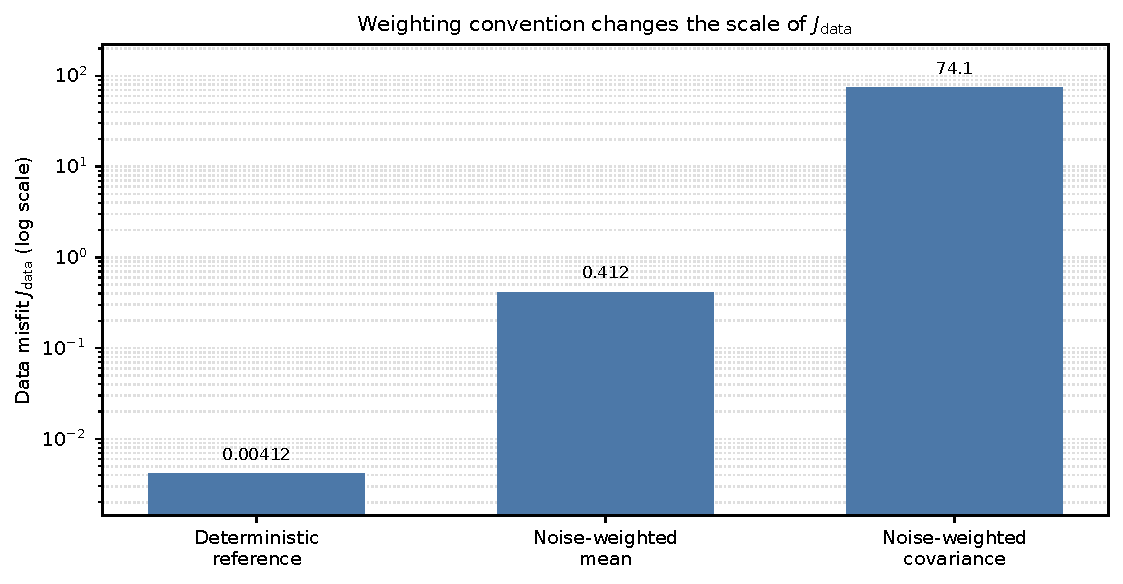
\includegraphics[width=0.47\textwidth]{appendices/figs_016_objective_weight_modes.pdf}
\caption{Effetto della convenzione di pesatura sul termine dati $J_{\rm data}$ per il parametro vero sintetico $\theta^\dagger$, rumore nominale $\eta=10\%$ e $\lambda=10^{-4}$. I valori sono $4.119\times10^{-3}$ (riferimento deterministico), $0.4119$ (noise-weighted mean) e $74.144$ (covarianza inversa esatta). Il termine di regolarizzazione resta $4.363\times10^{-6}$; le scale del costo dati, e quindi il compromesso con la penalizzazione, dipendono dalla convenzione.}
\end{figure}
\begin{figure*}[t]
\centering
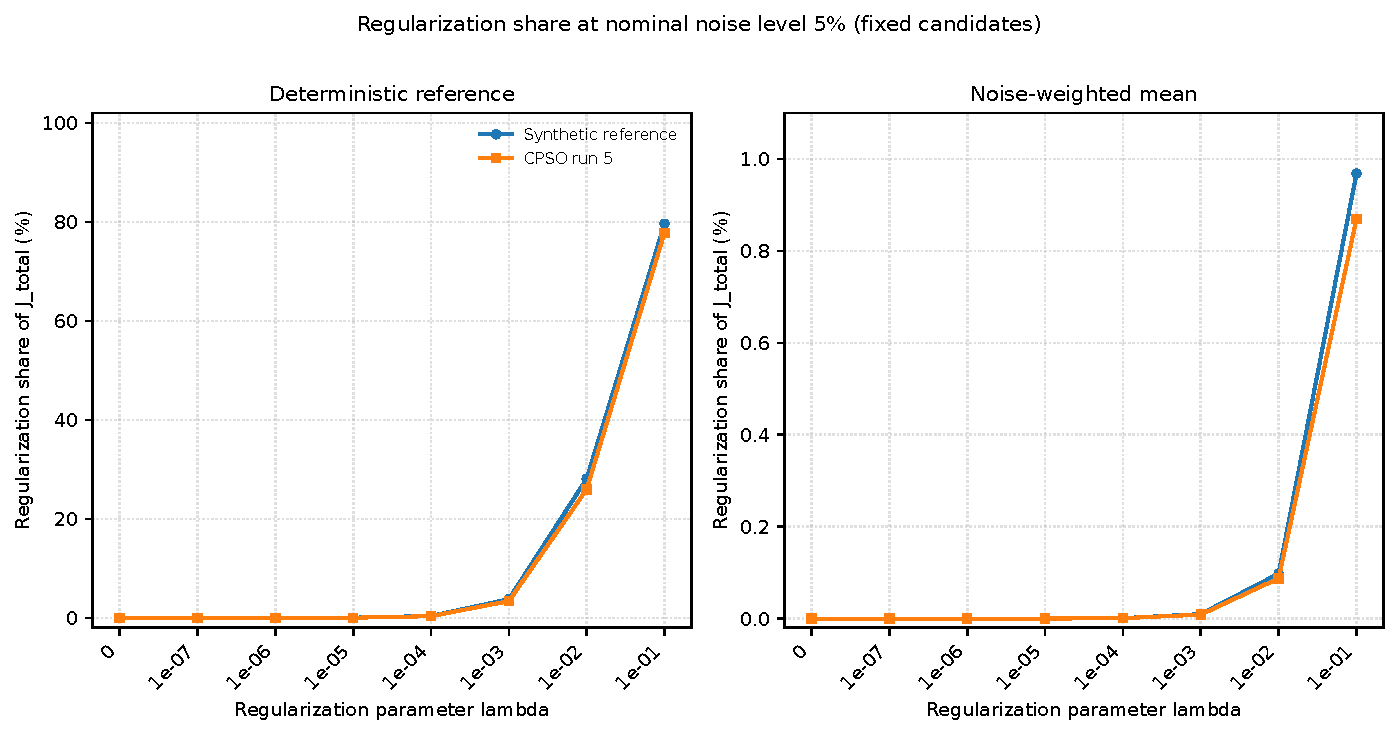
\includegraphics[width=0.94\textwidth]{appendices/figs_017_lambda_grid.pdf}
\caption{Quota del termine di regolarizzazione nel costo totale in funzione di $\lambda$, al livello nominale di rumore del 5\%, per due candidati fissati. I pannelli usano scale verticali distinte per rendere leggibili entrambe le convenzioni: i valori non vanno confrontati come se condividessero la stessa scala. La figura è una valutazione diagnostica del funzionale, non una curva di ottimizzazione.}
\end{figure*}

\subsection{Verifica della conversione di scala usata nella campagna finale}

Nella campagna finale rumorosa si impiega Mode B covariance, cioè $W^{\mathsf T}W=\Sigma^{-1}=\sigma^{-2}I$, con $N_{\rm obs}=180$ e scala di riferimento $\eta_{\rm ref}=0.05$. Il valore di conversione equivalente a un dato livello $\eta$ è
\[
\lambda_B^{\rm eq}(\eta)=\frac{N_{\rm obs}}{\eta^2}\lambda_A.
\]
Pertanto, con $\lambda_A=10^{-4}$, si ottiene $\lambda_B^{\rm eq}(0.05)=7.2$, mentre $\lambda_B^{\rm eq}(0.10)=1.8$. Nel protocollo congelato è stato mantenuto $\lambda_B=7.2$ per entrambe le classi rumorose. Questa scelta conserva l'equivalenza di scala soltanto a $\eta=0.05$; a $\eta=0.10$ la regolarizzazione ha peso relativo quattro volte maggiore rispetto a quello del protocollo equivalente. Non è quindi corretto attribuire le differenze osservate tra i due gruppi esclusivamente all'aumento del rumore. Il contratto numerico è stato testato prima di eseguire le run rumorose.

\begin{table}[H]
\centering
\caption{Audit numerico della conversione di scala nella campagna finale, valutato sul medesimo residuo di prova.}
\label{tab:normalization-contract}
\small
\begin{tabular}{lr}
\toprule
Controllo & Valore osservato\\
\midrule
Fattore atteso $N_{\rm obs}/\eta_{\rm ref}^2$ & $72000$\\
Rapporto $J_{\rm data}^{B}/J_{\rm data}^{A}$ & $72000$\\
Rapporto $J_{\rm reg}^{B}/J_{\rm reg}^{A}$ & $72000$\\
Rapporto $J_{\rm total}^{B}/J_{\rm total}^{A}$ & $72000$\\
Isolamento del target pulito & verificato\\
Decomposizione $J_{\rm total}=J_{\rm data}+J_{\rm reg}$ & verificata\\
\bottomrule
\end{tabular}
\end{table}

La conversione rende equivalente il rapporto fra termine dati e regolarizzazione al livello di riferimento $\eta_{\rm ref}=0.05$ per il residuo usato nel controllo. La stessa costante $\lambda_B$ è stata poi mantenuta per entrambe le classi rumorose; poiché $\sigma$ dipende dal livello $\eta$, il bilanciamento relativo non è esattamente invariato tra $\eta=0.05$ e $\eta=0.10$. Questa scelta è da documentare e non deve essere descritta come una calibrazione automatica ottimale della regolarizzazione.
